%\documentclass[useAMS,usenatbib,fleqn,dvipdfm]{emulateapj-rtx4}
%\documentclass[fleqn,dvipdfmx]{emulateapj-rtx4}
\documentclass[fleqn,dvipdfmx]{article}

%\usepackage[dvipdfm]{graphicx,color}
%\usepackage{amssymb}
\usepackage{amsmath}
%\usepackage{ulem}
\usepackage{bm}
\usepackage{color}
\usepackage{graphicx}

\newcommand{\jcop}{Journal of Computational Physics}
\newcommand{\sci}{Science}

\newcommand{\redtext}[1]{\textcolor{red}{#1}}
\newcommand{\bluetext}[1]{\textcolor{blue}{#1}}

\newcommand{\gcm}{\mbox{g~cm}^{-3}}
\newcommand{\cms}{\mbox{cm s}^{-1}}
\newcommand{\ergs}{\mbox{erg s}^{-1}}
\newcommand{\ergcms}{\mbox{erg cm}^{-2}~\mbox{s}^{-1}}
\newcommand{\cowd}{CO~WD }
\newcommand{\cowds}{CO~WDs }

\newcommand{\mdlx}[1]{$#1$M}
\newcommand{\vej}{v_{\rm ej}}
\newcommand{\tta}{t_{3\alpha}}
\newcommand{\ttar}{t_{3\alpha, {\rm r}}}
\newcommand{\ttas}{t_{3\alpha, {\rm s}}}
\newcommand{\tcc}{t_{\rm cc}}
\newcommand{\tccr}{t_{\rm cc,r}}
\newcommand{\tccs}{t_{\rm cc,s}}
\newcommand{\tdy}{t_{\rm dyn}}
\newcommand{\deta}{\epsilon_{3\alpha}}
\newcommand{\decc}{\epsilon_{\rm cc}}
\newcommand{\fsni}{$^{56}$Ni }
\newcommand{\fhe}{f_{\rm He}}

\newcommand{\km}[1]{{\bf{[KM: #1]}}}

%%%%%%%%%%%%%%%%%%%%%%%%%%%%%%%%%%%%%%%%%%%%%%%%

\begin{document}

\section{SPH w/ nuclear reaction}

Suppose we know acceleration, time derviative of energy, coefficient
viscosity, and the next timestep at the initial time. We integrate
each particle as follows:
\begin{enumerate}
\item Calculate the position, and predict the velocity and energy:
  \begin{align}
    \bm{r}_{i} &= \bm{r}^{(0)}_i + \bm{v}^{(0)}_i \Delta t +
    \frac{1}{2} \bm{a}^{(0)}_i \Delta t^2 \\
    %%
    \bm{v}^{(1/2)}_i &= \bm{v}^{(0)}_i + \frac{1}{2} \bm{a}^{(0)}
    \Delta t \\
    %%
    u^{(1/2)}_i &= u^{(0)}_i + \frac{1}{2} \dot{u}^{(0)} \Delta t
    \redtext{+ \epsilon_{{\rm nuc},i}(\Delta t/2)} \\
    %%
    \tilde{\bm{v}}_{i} &= \bm{v}^{(0)}_i + \bm{a}^{(0)}_i \Delta t \\
    %%
    \tilde{\bm{u}}_{i} &= \bm{u}^{(0)}_i + \dot{\bm{u}}^{(0)}_i \Delta
    t \redtext{+ \epsilon_{{\rm nuc},i}(\Delta t)} \\
    %%
    \tilde{\alpha}_i &= \alpha^{(0)}_i + \dot{\alpha}^{(0)}_i \Delta t,
  \end{align}
  \redtext{where ($\epsilon_{{\rm nuc},i}$) is energy generated
    through nuclear reaction. When the reaction is exothermic, the
    density and temperature are fixed at this time. On the other hand,
    when the reaction is endothermic, only the density is fixed at
    this time.}

%%%%%%%%%%%%%%%%%%%%%%%%%%%%%%%%%%%%%%%%%%%%%%%%%%%%%%%%%%%%%%%%%%%%%
\item Calculate the density, kernel-support length and grad-h term of
  each particle by an iterative method:
  \begin{enumerate}
  \item Estimate the density by the following
    expression: \label{item:estimatedensity}
    \begin{align}
      \rho_i &= \sum_j m_j W_i \\ \Omega_i &= 1 + \frac{1}{D}
      \frac{H_i}{\rho_i} \sum_j m_j \frac{\partial W_i}{\partial H_i}
    \end{align}
    where $W_i=W(r_{ij},H_i)$, $r_{ij}=|\bm{r}_{ij}|$, and
    $\bm{r}_{ij}=\bm{r}_i-\bm{r}_j$. The kernel function is expressed
    as
    \begin{align}
      W(r,H) &= H^{-D} w(r/H), \\ \frac{\partial
        W(r,H)}{\partial H} &= -H^{-(D+1)} \left[ D w(q) + q
        \frac{\partial w}{\partial q} \right].
    \end{align}
    The formula of $w(q)$ and $\partial w/\partial q$ are described in
    Appendix~\ref{sec:kernels}.
  \item calculate the kernel length as follow:
    \begin{align}
      H_i = \max \left[ (H/h) \times \eta \left( \frac{m_i}{\rho_i}
        \right)^{1/D}, H_{\max} \right],
    \end{align}
    where $h$ is the kernel length. Here, $H_{\max}$ is the initial
    distance of the binary separation, or the maximum \texttt{double}
    in the case of the single WD. The values of $\eta$ and $H/h$ are
    described in Appendix~\ref{sec:kernels}.
  \item Return to step~(\ref{item:estimatedensity}) unless this is the
    3rd time.
  \item Calculate divergence and rotation of $\bm{v}$:
    \begin{align}
      \nabla \cdot \tilde{\bm{v}}_i &= - \frac{1}{\Omega_i \rho_i} \sum
      \tilde{\bm{v}}_{ij} \cdot \left[ m_j \frac{\partial
          W_i}{\partial r_{ij}} \frac{\bm{r}_{ij}}{r_{ij}} \right], \\
%%
      \nabla \times \tilde{\bm{v}}_i &= \frac{1}{\Omega_i \rho_i} \sum
      \tilde{\bm{v}}_{ij} \times \left[ m_j \frac{\partial
          W_i}{\partial r_{ij}} \frac{\bm{r}_{ij}}{r_{ij}} \right].
    \end{align}
    The
    derivative of the kernel function is as follows:
    \begin{align}
      \frac{\partial W(r,H)}{\partial r} = H^{-(D+1)} \frac{\partial
        w(r/H)}{\partial (r/H)}.
    \end{align}
  \end{enumerate}
  
%%%%%%%%%%%%%%%%%%%%%%%%%%%%%%%%%%%%%%%%%%%%%%%%%%%%%%%%%%%%%%%%%%%%%
\item Calculate the pressure ($\tilde{P}_i$) and sound speed
  ($\tilde{c}_{{\rm s},i}$) as follows:
  \begin{align}
    P_i &= (\gamma - 1) \rho_i \tilde{u}_i \\
    c_{{\rm s},i} &= \left( \gamma \frac{P_i}{\rho_i} \right)^{1/2},
  \end{align}
  or Helmholtz EOS\redtext{, in which case the temperature
    ($\tilde{T}_i$) is also obtained}.

%%%%%%%%%%%%%%%%%%%%%%%%%%%%%%%%%%%%%%%%%%%%%%%%%%%%%%%%%%%%%%%%%%%%%
\item Calculate the Balsara switch:
  \begin{align}
    f_i &= \frac{|\nabla \cdot \tilde{\bm{v}}_i|}{|\nabla \cdot
      \tilde{\bm{v}}_i| + |\nabla \times \tilde{\bm{v}}_i| + 0.0001
      \tilde{c}_{{\rm s},i} / h_i}.
  \end{align}

%%%%%%%%%%%%%%%%%%%%%%%%%%%%%%%%%%%%%%%%%%%%%%%%%%%%%%%%%%%%%%%%%%%%%
\item Calculate the acceleration and the time derivative of the
  energy:
  \begin{align}
    \bm{a}_i &= - \sum \left( \frac{\tilde{P}_i}{\Omega_i \rho_i^2} +
    \frac{\tilde{P}_j}{\Omega_j \rho_j^2} + f_{ij} \Pi_{ij} \right)
    \left[ \frac{m_j}{2} \left( \frac{\partial W_i}{\partial r_{ij}} +
      \frac{\partial W_j}{\partial r_{ij}} \right)
      \frac{\bm{r}_{ij}}{r_{ij}} \right], \\ \dot{u}_i &= \sum \left(
    \frac{\tilde{P}_i}{\Omega_i \rho_i^2} + \frac{f_{ij} \Pi_{ij}}{2}
    \right) \left[ \frac{m_j}{2} \left( \frac{\partial W_i}{\partial
        r_{ij}} + \frac{\partial W_j}{\partial r_{ij}} \right)
      \frac{\bm{r}_{ij}}{r_{ij}} \right] \cdot \tilde{\bm{v}}_{ij},
  \end{align}
  where $f_{ij}=(f_i+f_j)/2$, and $\Pi_{ij}$ is an artificial
  viscosity. The artificial viscosity is expressed as follows:
  \begin{align}
    \Pi_{ij} &= - \frac{\tilde{\alpha}_i}{2} \frac{v_{ij}^{\rm sig}
      w_{ij}}{\rho_{ij}} \\
%%
    v_{ij}^{\rm sig} &= c_{{\rm s},i} + c_{{\rm s},j} - 3 w_{ij} \\
%%
    w_{ij} &= \left\{
    \begin{array}{ll}
      \displaystyle \frac{\bm{r}_{ij} \cdot
        \tilde{\bm{v}}_{ij}}{|\bm{r}_{ij}|} & (\bm{r}_{ij} \cdot
     \tilde{\bm{v}}_{ij} < 0) \\ 0 & (\bm{r}_{ij} \cdot
      \tilde{\bm{v}}_{ij} \ge 0)
    \end{array}
    \right.    
  \end{align}
  where $\rho_{ij}=(\rho_i+\rho_j)/2$.

%%%%%%%%%%%%%%%%%%%%%%%%%%%%%%%%%%%%%%%%%%%%%%%%%%%%%%%%%%%%%%%%%%%%%
\item Calculate $\dot{\alpha}$:
  \begin{align}
    \dot{\alpha}_i &= - \frac{\tilde{\alpha}_i - \alpha_{\rm
        min}}{h_i/(0.25\tilde{c}_{{\rm s},i})} + S_i \\ 
    %%
    S_i &= \max \left[ -(\nabla \cdot \tilde{\bm{v}}_i)(\alpha_{\rm
        max}-\tilde{\alpha}_i), 0 \right]
  \end{align}

%%%%%%%%%%%%%%%%%%%%%%%%%%%%%%%%%%%%%%%%%%%%%%%%%%%%%%%%%%%%%%%%%%%%%
\item Correct the velocity and energy:
  \begin{align}
    \bm{v}_i &= \bm{v}^{(1/2)}_i + \frac{1}{2} \bm{a}_i \Delta t \\
    %%
    u_i &= u^{(1/2)}_i + \frac{1}{2} \dot{u}_i \Delta t \redtext{+
      \epsilon_{{\rm nuc},i}(\Delta t / 2)} \\
    %%
    \alpha_i &= \alpha^{(1/2)}_i + \frac{1}{2} \dot{\alpha}_i \Delta
    t.
  \end{align}
  \redtext{When the reaction is exothermic, the density and
    temperature are fixed at this time. On the other hand, when the
    reaction is endothermic, only the density is fixed at this time.}

%%%%%%%%%%%%%%%%%%%%%%%%%%%%%%%%%%%%%%%%%%%%%%%%%%%%%%%%%%%%%%%%%%%%%
\item Calculate the next timestep:
%%  \begin{align}
%%    \Delta t = C \min_i \left[ \min \left( \frac{2H_i}{\max_j \left(
%%        v_{ij}^{\rm sig} \right) }, \frac{u_i}{|\dot{u}_i|} \right)
%%      \right].
%%  \end{align}
  \begin{align}
    \Delta t_{\rm next} = C \min_i \left[ \frac{2H_i}{\max_j \left(
        v_{ij}^{\rm sig} \right) }, \redtext{\Delta t \left|
        \frac{u_i^{(0)}}{u_i-u_i^{(0)}} \right|} \right].
  \end{align}

%%%%%%%%%%%%%%%%%%%%%%%%%%%%%%%%%%%%%%%%%%%%%%%%%%%%%%%%%%%%%%%%%%%%%
\item Return to step~1.
\end{enumerate}

\section{Helmholtz EOS}

Coorporate Timmes's EOS. The compositions are 100~\% carbon, 50~\%
carbon and 50~\% oxygen, and will be 100~\% helium.

\appendix

\section{Kernels}
\label{sec:kernels}

\subsection{Cubic spline kernel}

We describe the cubic spline kernel:
\begin{align}
  w(r/H) &= 2^D \sigma \times \left\{
  \begin{array}{ll}
    \left( 1 - 6 q^2 + 6 q^3 \right) & (0 \le q < 1/2) \\
%%
    \left[ 2 (1 - q)^3 \right] & (1/2 \le q < 1) \\
%%
    0 & (q \ge 1)
  \end{array}
  \right. \label{eq:cubicspline0-1} \\
%%
  \frac{\partial w(q)}{\partial q} &= (-6) 2^D \sigma
  \times \left\{
  \begin{array}{ll}
    1/3 & (0 \le q < 1/3) \\
%%
    \left(2q - 3q^2 \right) & (1/3 \le q < 1/2) \\
%%
    (1 - q)^2 & (1/2 \le q < 1) \\
    0 & (q \ge 1)
  \end{array}
  \right., \label{eq:cubicspline0-2}
\end{align}
where $\sigma = 2/3$ (1D), $10/7\pi$ (2D), and $1/\pi$ (3D).

For this kernel, $\eta=1.2$, and $H/h=2$.

The equations~(\ref{eq:cubicspline0-1}) and (\ref{eq:cubicspline0-2})
can be rewritten as
\begin{align}
  w(r/H) &= 2^D \sigma \times 2 \left[ (1-q)^3_+ - 4 (1/2 - q)^3_+
    \right], \\
%%
  \frac{\partial w(q)}{\partial q} &= (-6)2^D \sigma \times \left[
    (1-q)^2_+ - 4(1/2-q)^2_+ + 3(1/3-q)^2_+) \right],
\end{align}
where $(x)_+ \equiv \max(0, x)$.

\subsection{Wendland C$^2$ kernel}

We describe Wendland C$^2$ kernel: In the case of $D = 1$,
\begin{align}
  w(q) &= C_{\rm W} (1-q)_+^3 (1+3q) \\ \frac{\partial w(q)}{\partial
    q} &= 3 C_{\rm W} \left[(1-q)^3_+ - (1-q)^2_+ (1+3q) \right],
\end{align}
and in the case of $D = 2, 3$,
\begin{align}
  w(q) &= C_{\rm W} (1-q)_+^4 (1+4q) \\ \frac{\partial w(q)}{\partial
    q} &= 4 C_{\rm W} \left[(1-q)^4_+ - (1-q)^3_+ (1+4q) \right],
\end{align}
where $C_{\rm W}=5/4$ ($D=1$), $7/\pi$ ($D=2$), and $21/(2\pi)$
($D=3$). For this kernel, $\eta=1.6$, and $H/h=1.620185(D=1)$,
$1.897367(D=2)$, and $1.93492(D=3)$.

\subsection{Wendland C$^4$ kernel}

We describe Wendland C$^4$ kernel: In the case of $D = 1$,
\begin{align}
  w(q) &= C_{\rm W} (1-q)_+^5 (1+5q+8q^2) \\
%%
  \frac{\partial w(q)}{\partial q} &= C_{\rm W} (1-q)_+^4 \left[
    -5(1+5q+8q^2) + (1-q)_+ (5+16q) \right]
\end{align}
and in the case of $D = 2, 3$,
\begin{align}
  w(q) &= C_{\rm W} (1-q)_+^6 \left[ 1+6q+(35/3)q^2 \right] \\
%%
  \frac{\partial w(q)}{\partial q} &= C_{\rm W} (1-q)_+^5 \left\{-6
  \left[ 1+6q+(35/3)q^2 \right] + (1-q)_+ \left[ 6+(70/3)q \right]
  \right\}
\end{align}
where $C_{\rm W}=3/2$ ($D=1$), $9/\pi$ ($D=2$), and $495/(32\pi)$
($D=3$). For this kernel, $\eta=1.6$, and $H/h=1.936492(D=1)$,
$2.171239(D=2)$, and $2.207940(D=3)$.

\section{SPH tests}

\begin{enumerate}
\item 1D shock tube (CUBICSPLINE, USE\_AT1D)
\item 3D shock tube (CUBICSPLINE)
\item Strong shock (CUBICSPLINE, USE\_AT1D)
\item Point like explosion (CUBICSPLINE)
\item Evrard test (CUBICSPLINE, USE\_AT3D, GRAVITY)
\end{enumerate}

\begin{figure}
  \begin{center}
    \includegraphics[width=10cm,bb=0 0 1020 840]{fig/shock_1d/draw.png}
  \end{center}
  \caption{1D shock tube (cubic spline, $\gamma=1.4$, $\alpha=1.0$).}
\end{figure}

\begin{figure}
  \begin{center}
    \includegraphics[width=10cm,bb=0 0 1020 840]{fig/shock_3d/draw.png}
  \end{center}
  \caption{3D shock tube (cubic spline, $\gamma=1.4$, $\alpha=1.0$).}
\end{figure}

\begin{figure}
  \begin{center}
    \includegraphics[width=10cm,bb=0 0 1020 840]{fig/strong/draw.png}
  \end{center}
  \caption{Strong shock (cubic spline, $\gamma=1.4$, $\alpha=1.0$).}
\end{figure}

\begin{figure}
  \begin{center}
    \includegraphics[width=10cm,bb=0 0 1020 840]{fig/pex/draw.png}
  \end{center}
  \caption{Point like explosion (cubic spline, $\gamma=5/3$,
    $\alpha=3.0$).}
\end{figure}

\begin{figure}
  \begin{center}
    \includegraphics[width=14cm,bb=0 0 2120 2000]{fig/evrard/draw.png}
  \end{center}
  \caption{Evrard test (cubic spline, $\gamma=5/3$, $\alpha_{\rm
      min}=0.1$, $\alpha_{\rm max}=3.0$).}
\end{figure}

\section{EOS tests}

\begin{figure}
  \begin{center}
    \includegraphics[width=14cm,bb=0 0 980 480]{fig/eos/draw.png}
  \end{center}
  \caption{Helmholtz EOS w/ lookup table (top) and w/o (bottom).}
\end{figure}

\begin{figure}
  \begin{center}
    \includegraphics[width=10cm,bb=0 0 520 480]{fig/wdeq/draw.png}
  \end{center}
  \caption{Single COWD equilibrium ($1k/0.1M_{\odot}$) w/ new
    damping. The new damping mode is the addtion of a sort of cooling
    during 100 s, such that $u_{{\rm new},i} = (u_{{\rm old},i} -
    u_{\rm min}(\rho_i)) \exp(-0.1 \Delta t) + u_{\rm min}(\rho_i)$.}
\end{figure}

\begin{figure}
  \begin{center}
    \includegraphics[width=14cm,bb=0 0 880 480]{fig/bwd.1.8_he1e-1/draw.png}
  \end{center}
  \caption{Density and temperature of $1.1M_\odot$ and $1.0M_\odot$
    COWDs ($1k/0.1M_{\odot}$) from $1.8 \times 10^9$cm. Blue points
    indicate helium particles ($f_{\rm He}=0.1$).}
\end{figure}

\begin{figure}
  \begin{center}
    \includegraphics[width=14cm,bb=0 0 880 1200]{fig/wddamp/draw.png}
  \end{center}
  \caption{$1M_\odot$ COWD ($1k/0.1M_{\odot}$).}
\end{figure}

\begin{figure}
  \begin{center}
    \includegraphics[width=14cm,bb=0 0 1000 960]{fig/wddamp/draw2.png}
  \end{center}
  \caption{$1M_\odot$ COWD ($1k/0.1M_{\odot}$).}
\end{figure}

\begin{figure}
  \begin{center}
    \includegraphics[width=14cm,bb=0 0 880 1240]{fig/bwd.1.8/draw.png}
  \end{center}
  \caption{Density and temperature of $1.1M_\odot$ and $1.0M_\odot$
    COWDs ($1k/0.1M_{\odot}$) from $1.8 \times 10^9$cm.}
\end{figure}

\begin{figure}
  \begin{center}
    \includegraphics[width=14cm,bb=0 0 880 1240]{fig/bwd.1.5/draw.png}
  \end{center}
  \caption{Density and temperature of $1.1M_\odot$ and $1.0M_\odot$
    COWDs ($1k/0.1M_{\odot}$) from $1.5 \times 10^9$cm.}
\end{figure}

\end{document}
